% =====================================================================
%  F21DL Data Mining and Machine Learning - Group Coursework
%  Group 15 - Final report
%  Build:  pdflatex main.tex  (twice, for cross-references)
%  Layout: IEEEtran journal, A4, 11 pt body (the brief's minimum),
%          margins >= 1.27 cm on all four sides.
% =====================================================================
\documentclass[11pt,journal,a4paper]{IEEEtran}

\usepackage[T1]{fontenc}
\usepackage[utf8]{inputenc}
\usepackage{graphicx}
\usepackage{booktabs}
\usepackage{amsmath}
\usepackage{array}
\usepackage[table]{xcolor}
\usepackage{url}
\usepackage[hidelinks]{hyperref}
\usepackage{needspace}
\usepackage{caption}

\graphicspath{{figures/}}

% Captions and table bodies are set at 11 pt, the smallest size the brief allows.
\DeclareCaptionFont{elev}{\fontsize{11}{13}\selectfont}
\captionsetup{font={elev},labelfont=bf,labelsep=period}
\newcommand{\tabfont}{\fontsize{11}{13}\selectfont}

\setlength{\textfloatsep}{8pt plus 2pt minus 2pt}
\setlength{\intextsep}{7pt plus 2pt minus 2pt}
\setlength{\abovecaptionskip}{4pt}
\setlength{\belowcaptionskip}{2pt}


% Pack floats tightly so the six-page limit is spent on content, not white space.
\renewcommand{\topfraction}{0.92}
\renewcommand{\bottomfraction}{0.6}
\renewcommand{\textfraction}{0.06}
\renewcommand{\floatpagefraction}{0.75}
\renewcommand{\dbltopfraction}{0.92}
\renewcommand{\dblfloatpagefraction}{0.75}
\setcounter{topnumber}{3}
\setcounter{dbltopnumber}{2}
\setcounter{totalnumber}{4}

% Long unbreakable \texttt tokens in a narrow column otherwise force one word per line.
\setlength{\emergencystretch}{3em}
\hyphenpenalty=200
\begin{document}

% =====================================================================
% 0. TITLE PAGE
% =====================================================================
\begin{titlepage}
\centering
\vspace*{2.6cm}

{\fontsize{11}{13.2}\selectfont F21DL Data Mining and Machine Learning --- Group Coursework, 2026--2027\par}

\vspace{2.4cm}

\rule{\textwidth}{1.2pt}
\vspace{0.7cm}

{\LARGE\bfseries Telling Fake Websites from Real Ones\par}
\vspace{10pt}
{\large Detecting Phishing Pages from Tabular Evidence and Screenshots\par}

\vspace{0.7cm}
\rule{\textwidth}{1.2pt}

\vspace{2.8cm}

{\large\bfseries Group 15\par}
\vspace{0.55cm}
{\normalsize Repository: \url{https://github.com/Sakib-Dalal/DMML-F21DL-CourseWork01-PG-Group15}\par}

\vspace{2.4cm}

{\renewcommand{\arraystretch}{1.5}
\begin{tabular}{ll}
\toprule
\textbf{Full name} & \textbf{Matriculation number} \\
\midrule
Arafa Mehar        & H00561458 \\
Syed Umraaz        & H00557679 \\
Sakib Dalal        & H00549861 \\
Eric Lazar Antony  & H00549103 \\
Rishab Dhinesh     & H0058666 \\
\bottomrule
\end{tabular}\par}

\vfill
\end{titlepage}

% =====================================================================
% BODY
% =====================================================================
\pagestyle{plain}

\noindent{\fontsize{11}{13.2}\selectfont\itshape\textbf{Abstract}---A phishing page copies somebody else's
login page to collect a password that does not belong to it. We ask whether the address a page sits on, or the way
the page \emph{looks}, is the stronger evidence that it is fake. We answer it with one protocol across three
published, freely licensed datasets: 235{,}370 unique websites described by 50 page measurements, and 61{,}375
cleaned screenshots. After removing three columns that restate the answer, we train six supervised models, two
clusterers and four convolutional networks. The tabular models reach 0.9944 to 0.9996 accuracy on 70{,}611 held-out
websites; the screenshot networks reach 0.8750 to 0.8962 on 2{,}400 images, a gap of about ten points. Page
measurements outrank address measurements, and a three-question tree still reaches 0.9896. Most surprising, a
Gaussian mixture recovers the classes with an adjusted Rand index of 0.985 and no labels, which says more about the
corpus than about detection.\par}
\normalsize
\vspace{3pt}

% ---------------------------------------------------------------------
\section{Introduction}
% ---------------------------------------------------------------------

A phishing page is a copy of a login page somebody else owns, put online to collect a password, a card number or a
one-time code. Page savers and free hosting make a convincing clone an afternoon's work, and it can be used and
abandoned before a blocklist catches up. Because the page is a copy, the victim is not asked to trust a stranger but
to log in to a service they already use, which is why phishing endures as one of the most reported forms of
cybercrime \cite{khonji2013phishing,basit2021comprehensive}.

The problem is three problems, because three teams act on the verdict. A browser vendor needs an answer in the
time it takes to paint a page, with no GPU available. A security analyst needs to know \emph{why} a page was
blocked, because an unexplained block gets appealed. A bank needs to know how many blocks are real, because a
false alarm sends a customer into a telephone queue. Accuracy answers none of that, so we report precision,
recall, latency and cost beside it.

Research has followed the available evidence rather than the problem, in three lines. One reads the address
string: its length, digits, hyphens and sub-domains
\cite{sahingoz2019ml,rao2019detection,marchal2014phishstorm}. One reads the page source: links pointing
off-site, forms posting to third parties, copyright lines \cite{rao2019detection,fette2007learning}. One reads
the picture, on the argument that an attacker must copy the look of a page and rarely the address
\cite{lin2021phishpedia}. All three report scores near or above 0.95, which is suspicious: a detector scoring
0.999 on a random split of a crawled corpus is not necessarily one that scores 0.999 on tomorrow's pages
\cite{marchal2014phishstorm}. What is missing is not another detector but a comparison: tabular and visual
evidence are rarely put against each other under one protocol, unsupervised separation is rarely reported, and
the trade-off between the best score and the most explainable model is usually settled in favour of the
score.

\textbf{RQ1: can a model separate phishing from legitimate pages using tabular evidence, and how well?}
\emph{Hypothesis 1: yes, above 0.95.} We take 0.95 from the published baselines, which report above 0.97 from
URL words alone \cite{sahingoz2019ml} and near-perfect scores from selected address and page features
\cite{rao2019detection}; our file measures the page as well, so it should be no harder. It fails if no model
clears 0.95.

\textbf{RQ2: is the address or the page the stronger evidence?} \emph{Hypothesis 2: the page.} The argument is
attacker cost. A URL can be shortened, hyphenated or pushed behind HTTPS in minutes, precisely the weakness
Khonji \emph{et al.} name: features cheap for us to compute are cheap to imitate \cite{khonji2013phishing}. A
credible reference count, a description, social links and a realistic quantity of code are outputs of a real
publishing pipeline, and Fette \emph{et al.} found the same asymmetry in email, where structural evidence
outlived lexical evidence \cite{fette2007learning}. It fails if address features dominate both rankings and the
tree.

\textbf{RQ3: can clustering recover the two classes without labels?} \emph{Hypothesis 3: no, not well.} We
expected failure for two reasons: detection is treated throughout as supervised \cite{basit2021comprehensive},
and cluster analysis of mixed binary and count features tends to split on the largest difference in scale rather
than on meaning. Our bar is an adjusted Rand index (ARI) of 0.5. It fails if either algorithm clears it.

\textbf{RQ4: can a page be judged from its screenshot alone?} \emph{Hypothesis 4: partly, and worse than the
table.} A screenshot keeps layout, colour and logos and loses the address, the text and the HTML. Phishpedia
shows pixels carry real signal, but its method matches maintained brand references \cite{lin2021phishpedia}, a
narrower question than deciding whether a page is honest. It fails if the picture models match the tabular ones.

% ---------------------------------------------------------------------
\section{Related Work}
% ---------------------------------------------------------------------

\emph{Classical detection treats a page as a vector of measurements.} Sahingoz \emph{et al.}
\cite{sahingoz2019ml} compared seven classifiers on URL words and reported above 0.97 with a random forest,
establishing both the strength of the signal and the convention of measuring it by accuracy on a random split.
Rao and Pais \cite{rao2019detection} built a larger set from address and page source, selected it with a wrapper,
and reported near-perfect scores; their feature list is the ancestor of our four families. Marchal \emph{et al.}
\cite{marchal2014phishstorm} took the idea to stream scale, which is the setting a browser faces. Khonji
\emph{et al.} \cite{khonji2013phishing} name the weakness rather than the strength: features cheap to compute
are cheap to imitate, and features hard to imitate are expensive at browse time. 

\emph{Structure beats strings.} Fette \emph{et al.} \cite{fette2007learning} found that structural evidence
generalised better than lexical evidence in email, because structure is a by-product of the tooling that builds real
messages, which is why feature-based detectors generalise better than string-only ones
\cite{basit2021comprehensive}.

\emph{Pixels make the strongest narrow case.} Phishpedia \cite{lin2021phishpedia} abandons the URL blocklist and
matches logo and layout against protected brands, fast enough for live traffic, on the argument that an attacker
controls the address but must copy the appearance. The cost is a brand reference set to maintain and a blind
spot for pages imitating no known brand. Transfer learning from ImageNet backbones
\cite{he2016deep,tan2019efficientnet,howard2019searching} is the standard way to get a usable visual classifier
from a few thousand images, and it is the recipe we follow.

\emph{Corpus design is a hidden variable.} PhiUSIIL \cite{prasad2024phiusiil} is a good modern corpus: large,
licensed, and crawled from two kinds of source, which is what makes it usable and also what makes it separable.
Its authors report the problem we met, that some columns compare the URL against the page title or domain and so
nearly encode the label; a model that keeps them learns the rule that built the dataset. Marchal \emph{et al.}
\cite{marchal2014phishstorm} raise the second design problem, drift: phishing changes every quarter, so a random
split over one crawl flatters every model trained on it. Three things are therefore absent from this literature,
and our experiments are organised around them: a head-to-head of tabular and visual evidence under one protocol
(RQ1 against RQ4), any report of unsupervised separation (RQ3), and a measured cost for choosing the explainable
model over the most accurate one (RQ2 and Section~\ref{sec:disc}).

% ---------------------------------------------------------------------
\section{Dataset Description and Analysis}
% ---------------------------------------------------------------------

We use two views of one problem, drawn from three published datasets. Table~\ref{tab:data} gives their source,
licence and shape.

\begin{table*}[!t]
\centering
\caption{The datasets used, with their licences. Neither the raw tables nor the screenshots are
redistributed; only derived tables and figures appear here.}
\label{tab:data}
\tabfont
\setlength{\tabcolsep}{4pt}
\begin{tabular}{@{}>{\raggedright\arraybackslash}p{1.2cm}>{\raggedright\arraybackslash}p{4.4cm}>{\raggedright\arraybackslash}p{7.2cm}>{\raggedright\arraybackslash}p{2.7cm}@{}}
\toprule
\textbf{View} & \textbf{Source} & \textbf{Content and shape} & \textbf{Licence} \\
\midrule
Tabular &
PhiUSIIL Phishing URL dataset, UCI Machine Learning Repository, ID 967 \cite{prasad2024phiusiil} &
235{,}795 websites $\times$ 56 columns, 235{,}370 after de-duplication. One row per site: the address, then
counts and flags from the page source. Target \texttt{label}: 1 legitimate, 0 phishing. &
CC BY 4.0 \\
\addlinespace
Visual &
Zenodo, \emph{Phishing and Legitimate Websites Dataset}, v2.0, DOI 10.5281/zenodo.23477065
\cite{yadav2026zenodo}, merged with the Phishpedia benchmark of Lin \emph{et al.} \cite{lin2021phishpedia} &
91{,}740 raw screenshots (21{,}311 Zenodo, 70{,}429 Phishpedia); 61{,}375 after cleaning, then 8{,}000 per
class. RGB, resized to $224\times224$. &
CC BY 4.0 (Zenodo); research use (Phishpedia) \\
\bottomrule
\end{tabular}
\end{table*}

Of the 56 columns, 50 are numeric measurements, four are text (\texttt{URL}, \texttt{Domain}, \texttt{TLD},
\texttt{Title}), one is an identifier and one the target. The measurements fall into four families.
\emph{Address} columns describe the string (\texttt{URLLength}, \texttt{DegitRatioInURL}, \texttt{IsHTTPS}).
\emph{Content} columns count what the page holds (\texttt{NoOfImage}, \texttt{NoOfJS}, \texttt{LineOfCode}).
\emph{Trust} columns are flags an analyst checks by eye (\texttt{HasCopyrightInfo}, \texttt{HasSocialNet}).
\emph{Similarity} columns compare address against page, such as \texttt{URLSimilarityIndex}.

Cleaning found little to fix and one thing to fear. There are 425 duplicate addresses, no missing values and no
constant column. We dropped the four identifier columns, because a URL or file name is a memory of the training set
rather than a property of the page, and label-encoded the top-level domain (695 levels). That left 52 numeric columns
and 235{,}370 unique websites: 134{,}850 legitimate (57.3~\%) and 100{,}520 phishing (42.7~\%). A model that always
answers ``legitimate'' scores 0.5729, and every result below is read against that.

A first ranking put \texttt{URLSimilarityIndex} far ahead of everything else, which was a warning rather than a
result. Checked against the raw file, the column is exactly 100 for \emph{all} 134{,}850 legitimate websites and
for only 786 of the 100{,}945 phishing ones: it separates the classes because it restates the label, not because
similarity predicts phishing. The other two similarity columns behave the same way, with 98{,}439 legitimate
sites pinned at 100, so a model given them answers without looking at the page. We removed all three before any
model saw the data, and every score here is measured without them. This is the most important decision in the
study, and it is why our numbers sit below the values published for this dataset.

\emph{Exploratory analysis.} After removal the strongest signals are page-level flags, and URL length shows how
much easier the corpus is than the problem. Legitimate addresses occupy a narrow band, averaging 26.2 characters
with a maximum of 57; phishing addresses average 45.7 and reach 6{,}097, because a long tail carries query strings
and redirects (Fig.~\ref{fig:eda}, left). Such a clean separation is the signature of a corpus built from two
kinds of source, and the flags an analyst checks by eye separate the classes almost as sharply
(Fig.~\ref{fig:eda}, right). Correlation puts \texttt{HasSocialNet} (0.78), \texttt{HasCopyrightInfo} (0.74),
\texttt{HasDescription} (0.69) and \texttt{IsHTTPS} (0.61) first, while the strongest address measurement is
negative, \texttt{SpacialCharRatioInURL} at $-0.53$, then \texttt{DegitRatioInURL} at $-0.43$. The forest's
out-of-bag importance agrees on the first four, and we kept the 17 features both rankings
placed inside their top twenty. Only five describe the address string, so twelve measure the page before any
model is trained.

\begin{figure}[!t]
\centering
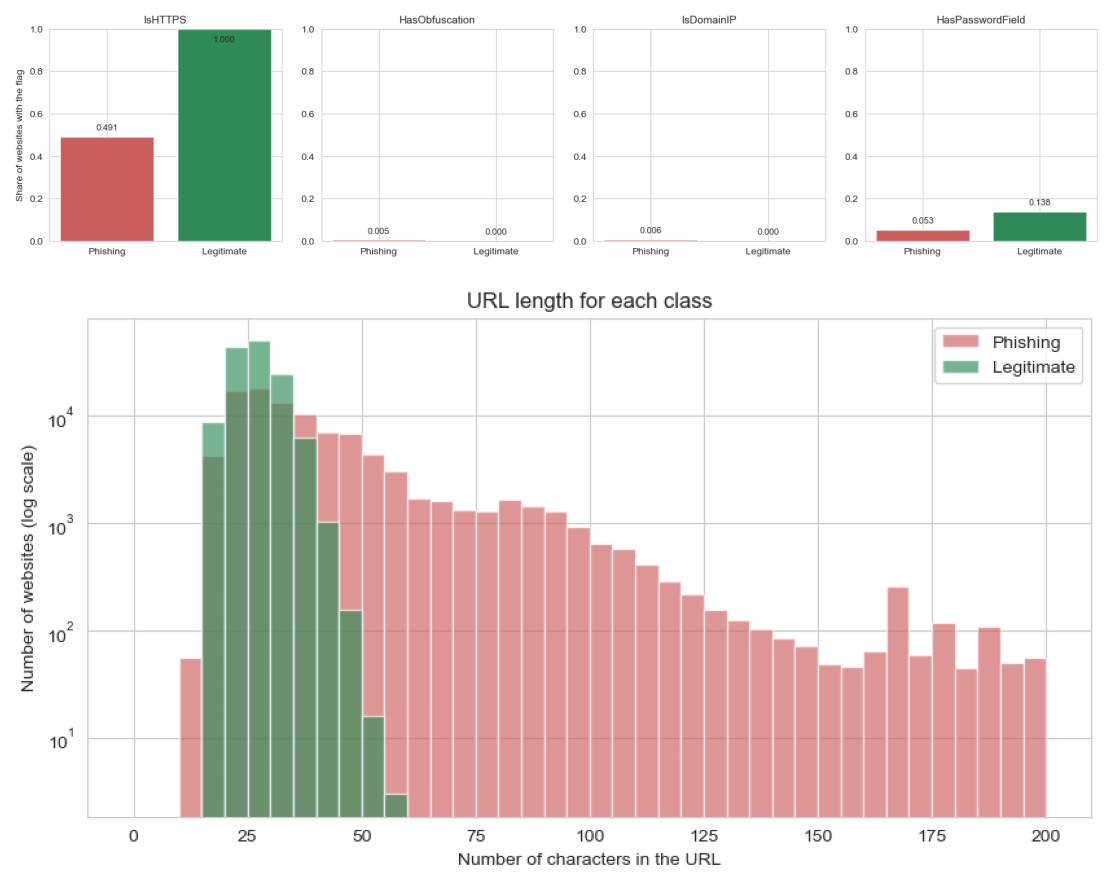
\includegraphics[width=0.93\columnwidth]{eda_tab}
\caption{Exploratory view before feature selection: (a) URL length by class on a log count axis;
(b) share of websites carrying each of four flags. Outputs of the tabular notebook.}
\label{fig:eda}
\end{figure}



\emph{The visual corpus needed real work.} Two sources contributed 91{,}740 indexed screenshots (Phishpedia
40{,}922 legitimate and 29{,}507 phishing; Zenodo 12{,}241 and 9{,}070). Auditing removed 30{,}365 in one pass
for three reasons applied together: files that would not decode, single-colour renders caught by a pixel standard
deviation below 1.0, and exact duplicates found by hashing a $64\times64$ RGB thumbnail. That left 61{,}375
images, but the classes were badly unequal, 50{,}945 legitimate against 10{,}430 phishing. A network trained on
that ratio learns the prior of the corpus rather than the look of a page, so we sampled 8{,}000 per class and
split 70/15/15 into 11{,}200 training, 2{,}400 validation and 2{,}400 test images at $224\times224$. Balancing
discards 42{,}945 legitimate images, a cost we accept knowingly: it trades redundant data for a test set whose
accuracy is interpretable.

The images are coarse in a way that matters for RQ4. Mean brightness is 180.7 for legitimate pages and 189.8 for
phishing, mean contrast 55.4 against 44.1, and edge strength 6.9 against 4.6: phishing pages are on average
brighter and flatter, though the distributions overlap heavily. At $224\times224$ a page 4{,}000 pixels tall is
compressed into a square, so two pages with the same header and different forms become almost the same image.
Both primary datasets are CC BY 4.0 and attributed in the bibliography; the Phishpedia benchmark is research-use
only, so it is neither redistributed nor used commercially. The screenshots contain real brand marks and
occasional personal data, so the corpus stays out of version control and no live site was visited.

% ---------------------------------------------------------------------
\section{Experimental Setup}
\label{sec:setup}
% ---------------------------------------------------------------------

\emph{Protocol.} We split the tabular data 70/30 with stratification, fitted every transformer on training rows only,
fixed the seed at 42 and touched the test rows once, so every supervised model saw the same 17 features and the same
70{,}611 websites. For the images, 2{,}400 validation images chose the epoch and 2{,}400 test images were scored
once.



\emph{Generative and discriminative coverage.} Both families are present, though not equally. Gaussian naive
Bayes is generative: it models class-conditional densities and applies Bayes' rule, which is why its
independence assumption fits badly here, where the flags are strongly correlated. The Gaussian mixture is
generative but stronger, fitted by expectation-maximisation \cite{dempster1977maximum}, the algorithm the
syllabus pairs with $k$-means. Everything else learns a boundary directly: logistic regression, $k$-nearest
neighbours, the decision tree and forest, the MLP and the four networks. The generative arm answers RQ3; the rest
answer RQ1, RQ2 and RQ4.

\emph{Why these nine models.} The five classical models are the standard spread for a tabular problem and each
fails differently: a linear boundary, a local vote, a strong independence assumption, a single axis-aligned tree
\cite{quinlan1986induction}, and an ensemble that averages many trees to cut variance \cite{breiman2001random}.
Including all five is what makes the near-identical scores in Section~\ref{sec:res} meaningful, because the
agreement is then between methods that share almost nothing.  The four networks cover RQ4 from both ends: one we designed, and three ImageNet
models \cite{he2016deep,tan2019efficientnet,howard2019searching} fine-tuned on the same head, so any difference is
architecture rather than training recipe.

\emph{Searching, without touching the test rows.} Every hyperparameter was chosen on a validation slice of the
training data, sweeping decision-tree depth from three to twenty, the minimum leaf size, the forest size, the
number of neighbours, the logistic penalty strength, and four MLP widths from one hidden layer to three. A
silhouette sweep over two to eight clusters selected two, at 0.310 against 0.274 for three. Two of those searches
became results in their own right, since the depth-three tree is 0.0090 behind the unconstrained one and the four
MLP widths are within 0.0002 of each other. Table~\ref{tab:cfg} lists the final settings.

\emph{The custom network.} Five convolutional blocks with 32, 64, 128, 256 and 256 filters, each a $3\times3$
convolution with batch normalisation and $2\times2$ max pooling, then a dense head of 256 and 128 units, GELU,
dropout 0.45 and a two-way output: 4{,}225{,}410 trainable parameters. It ran for 12 epochs with AdamW at
$3\times10^{-4}$, weight decay $3\times10^{-4}$, batch 64, cosine annealing to zero and label smoothing 0.1.
Inputs are resized to $224\times224$ and scaled to $[0,1]$; we applied no colour normalisation and no geometric
augmentation, in hindsight the weakest choice in the study.

\emph{The transfer baseline.} ResNet-18, MobileNetV3-Small and EfficientNet-B0 were loaded with ImageNet weights,
their final layer replaced by a two-way linear head, and fine-tuned end to end with no frozen blocks, for 8
epochs with Adam at $5\times10^{-4}$ and the same batch size, weight decay, input size and split. Holding the
recipe fixed is what lets us attribute Table~\ref{tab:img} to architecture. All image work ran on one NVIDIA
A100-SXM4-80GB; the tabular work ran on CPU, the deployment condition we care about.

% ---------------------------------------------------------------------
\section{Results}
\label{sec:res}

\emph{RQ1: classical models on the table.} Table~\ref{tab:class} gives the five classical models on the 70{,}611
held-out websites. All six clear 0.99; the weakest is Gaussian naive Bayes at 0.9944. The random forest leads the five
at 0.9995 accuracy and 0.9996 $F_1$; the MLP is a fraction ahead at 0.9996 and 0.9997. Precision and recall move
together in every row, so nobody buys accuracy by leaning on the majority: the largest gap between them is 0.0058,
in naive Bayes. In counts the MLP is wrong 28 times and naive Bayes 396, with the other four between.

\begin{table}[!t]
\centering
\caption{Classical and neural models on the tabular test set ($n=70{,}611$). Errors are counts on the same rows.}
\label{tab:class}
\tabfont
\setlength{\tabcolsep}{3.5pt}
\begin{tabular}{@{}lccccc@{}}
\toprule
\textbf{Model} & \textbf{Acc.} & \textbf{Prec.} & \textbf{Rec.} & \textbf{$F_1$} & \textbf{Err.} \\
\midrule
MLP (64,32,16)  & \textbf{0.9996} & \textbf{0.9996} & 0.9998 & \textbf{0.9997} & 28 \\
Random forest   & 0.9995 & 0.9994 & \textbf{0.9998} & 0.9996 & 34 \\
Decision tree   & 0.9986 & 0.9989 & 0.9986 & 0.9988 & 101 \\
Logistic regr.  & 0.9984 & 0.9983 & 0.9989 & 0.9986 & 112 \\
$k$-nearest (5) & 0.9978 & 0.9976 & 0.9986 & 0.9981 & 156 \\
Gaussian NB     & 0.9944 & 0.9922 & 0.9980 & 0.9951 & 396 \\
\bottomrule
\end{tabular}
\end{table}

The size of the gap is the result, not the winner: between the best and the worst model lie 0.0052 accuracy, about
368 websites, and a straight-line boundary lands within 0.0011 of 200 trees.

\emph{RQ2: which evidence ranks higher.} Address measurements appear in neither top four of either ranking. The tree
in Fig.~\ref{fig:tree} makes the mechanism legible rather than inferential: its first split asks whether the page
holds more than a threshold number of external references, the second whether the code exceeds a few hundred lines,
the third whether the page carries social links. All three are page-level, and the address enters only through the
density of special characters. Depth three costs 0.0090 against the unconstrained tree and buys a model that fits on a page and can be read
aloud; it reaches 0.9896 on test and 0.9888 on its own training rows, whereas the full tree is 0.9986 on test but
1.0000 on training. That is its practical case: three questions become three sentences an appeals team can cite, and a reviewer can change a threshold without retraining.

\begin{figure*}[!t]
\centering
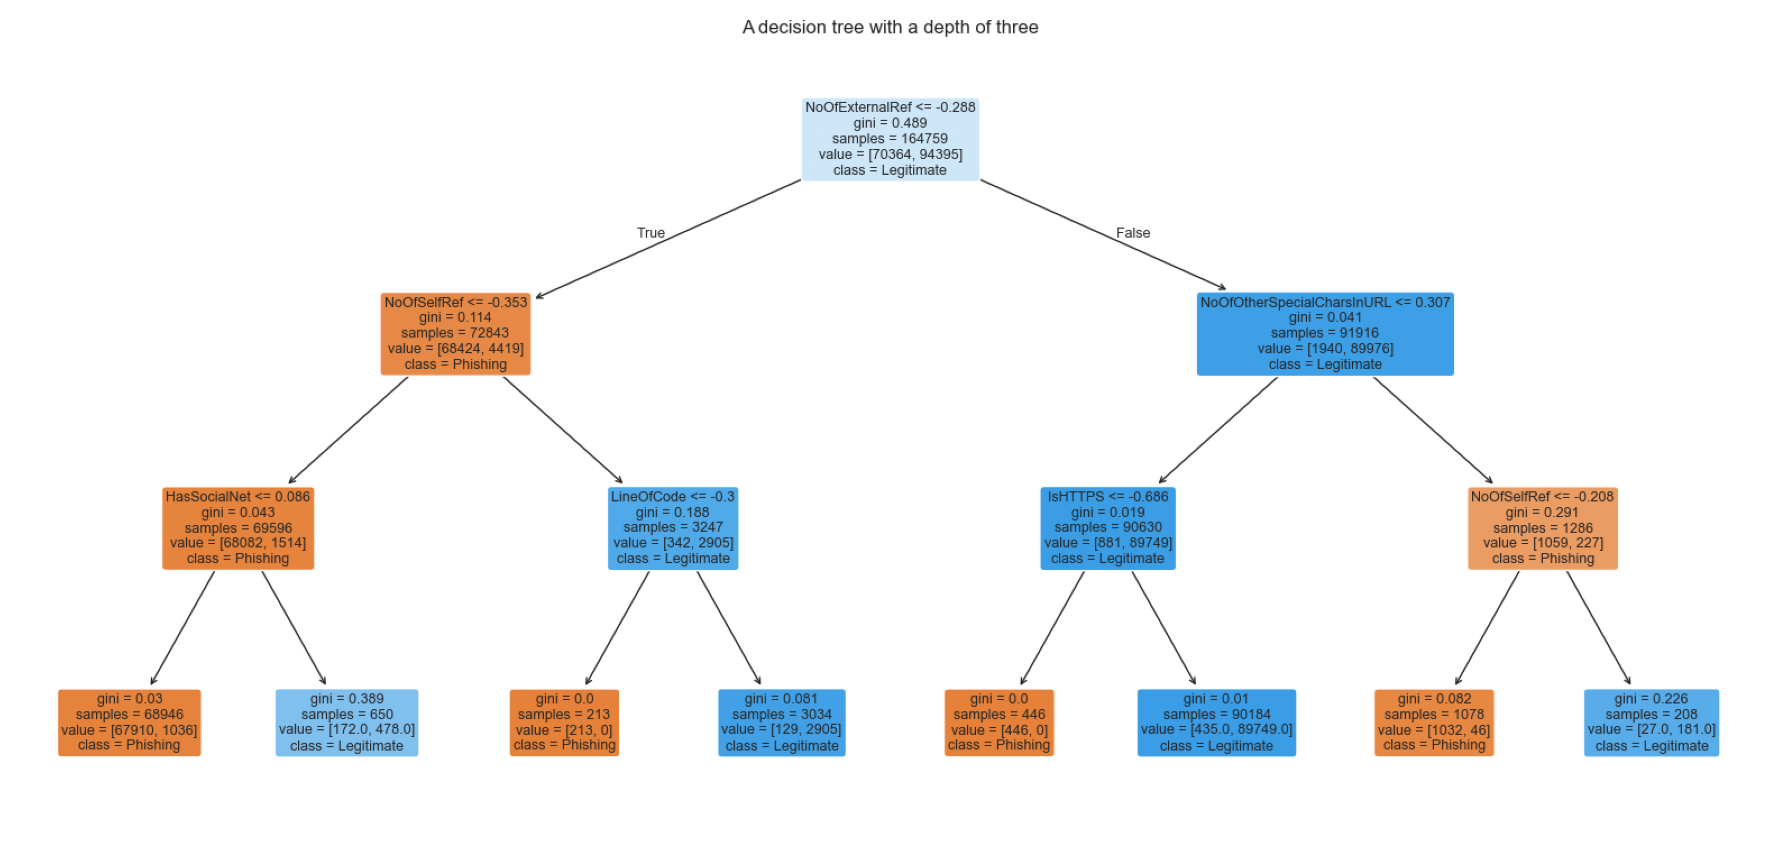
\includegraphics[width=0.78\textwidth]{tree_d3}
\caption{The depth-three decision tree. Nodes state the test, the Gini impurity and the sample count. The first
three questions are page-level, which answers RQ2 in one picture.}
\label{fig:tree}
\end{figure*}

\emph{RQ3: separation without labels.} Table~\ref{tab:clust} gives the two clusterers, both run with $k=2$ by
silhouette and both scored against labels they never saw. $k$-means reaches an ARI of 0.892 and the Gaussian mixture
0.985, close to a supervised result. The mixture's contingency table shows what that means: one group is almost
entirely legitimate and the other almost entirely phishing, with a few thousand websites on the wrong side of the
line.

\begin{table}[!t]
\centering
\caption{Unsupervised separation, scored against the true labels ($n=70{,}611$, $k=2$ by silhouette).}
\label{tab:clust}
\tabfont
\begin{tabular}{@{}lcc@{}}
\toprule
\textbf{Algorithm} & \textbf{ARI} & \textbf{NMI} \\
\midrule
$k$-means        & 0.892 & 0.824 \\
Gaussian mixture & \textbf{0.985} & \textbf{0.965} \\
\bottomrule
\end{tabular}
\end{table}

\emph{RQ4: the picture models.} Table~\ref{tab:img} gives the four networks on the 2{,}400 test screenshots.
EfficientNet-B0 is best at 0.8962 accuracy, 0.8974 $F_1$ and 0.9603 ROC-AUC. Our own network is second at 0.8925
with 4.23 million parameters, 0.0037 behind EfficientNet's 4.01 million; ResNet-18 is third at 0.8792 but needs
11.18 million, nearly three times ours; MobileNetV3-Small is last at 0.8750 with 1.52 million. All four sit inside a
0.0212 band while differing sevenfold in size, so the ceiling is the data rather than the architecture.

\begin{table*}[!t]
\centering
\caption{Screenshot models on the balanced test set ($n=2{,}400$). Time is training wall-clock on one A100; one
recipe and one split throughout.}
\label{tab:img}
\tabfont
\setlength{\tabcolsep}{4pt}
\begin{tabular}{@{}lcccccccc@{}}
\toprule
\textbf{Model} & \textbf{Acc.} & \textbf{Prec.} & \textbf{Rec.} & \textbf{Spec.} & \textbf{$F_1$} & \textbf{AUC} & \textbf{Param.} & \textbf{Time} \\
\midrule
EfficientNet-B0   & \textbf{0.8962} & 0.8875 & \textbf{0.9075} & 0.8850 & \textbf{0.8974} & \textbf{0.9603} & 4.01M & 2{,}861\,s \\
Custom CNN        & 0.8925 & 0.8925 & 0.8925 & \textbf{0.8925} & 0.8925 & 0.9535 & 4.23M & 4{,}263\,s \\
ResNet-18         & 0.8792 & \textbf{0.9106} & 0.8408 & 0.9175 & 0.8744 & 0.9471 & 11.2M & 2{,}821\,s \\
MobileNetV3-Small & 0.8750 & 0.8961 & 0.8483 & 0.9017 & 0.8716 & 0.9366 & 1.52M & 2{,}867\,s \\
\bottomrule
\end{tabular}
\end{table*}

Fig.~\ref{fig:curves} shows how our network trained, the clearest single summary of the visual task. Training
accuracy climbs to 0.9934 while validation accuracy stalls at 0.9012 from the eleventh epoch, so the gap widens to
0.0921; validation loss falls to 0.3210 and flattens. The network is memorising 11{,}200 images it has seen, not
learning layout that transfers to 2{,}400 it has not. The transient at epoch three, where validation accuracy drops
to 0.7392 before recovering, is a step a constant learning rate would not have survived.

\begin{figure}[!t]
\centering
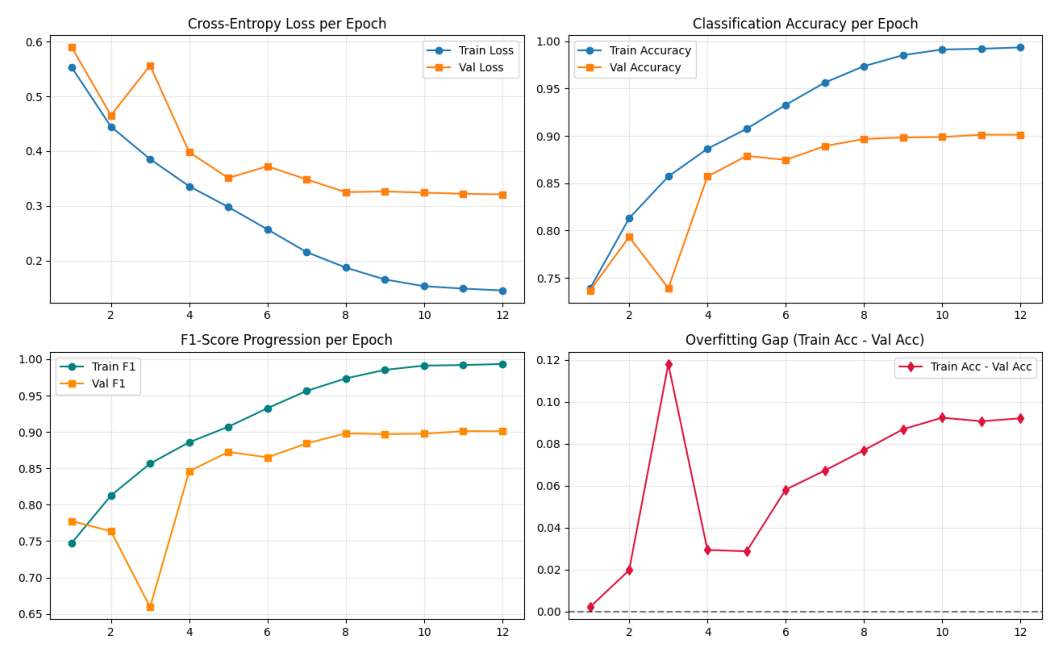
\includegraphics[width=0.95\columnwidth]{cnn_curves}
\caption{Training history of the custom CNN over 12 epochs. Validation accuracy plateaus at 0.9012 while training
accuracy reaches 0.9934.}
\label{fig:curves}
\end{figure}

The confusion matrix splits the 258 test errors evenly: 129 legitimate pages blocked and 129 phishing pages missed
out of 2{,}400, giving 1{,}071 correct on each side. That symmetry matters operationally, because the two errors
carry different costs. Most pages land at the extremes of the predicted-probability scale, but a band between 0.3
and 0.8 carries most of the errors.

\emph{Two further analyses.} Stratifying errors by source, the network got 182 of 1{,}850 Phishpedia images wrong
(9.8~\%) and 76 of 550 Zenodo images wrong (13.8~\%), so part of the error is domain shift between two capture
conventions. An interpretability pass showed early blocks responding to edges and text mass and later blocks to the
layout of a form; of five misclassified samples, four were legitimate pages rejected with high confidence, all of
them little more than a single centred form.

The two views do not meet. The best tabular model is 0.1034 accuracy above the best screenshot model, at matched
recall the table still wins, and the screenshot model's ROC-AUC of 0.9603 is below the tabular models' accuracy
before a threshold is chosen. Hypotheses 1, 2 and 4 are supported; Hypothesis 3 is refuted, and by a wide margin.

% ---------------------------------------------------------------------
\section{Discussion}
\label{sec:disc}

\emph{A near-perfect score is a property of the corpus.} The temptation is to read 0.9944 to 0.9996 as phishing
being nearly solved. These columns are not raw observations but the measurements an analyst would make, computed by
a crawler that had already visited both classes, so the file contains the analyst's reasoning and a supervised model
re-learns it easily. The strongest column was a similarity index that was 100 for every legitimate site; removing
that family cost us a perfect score and left a model measured against a fair question. This is the warning in the
survey literature \cite{khonji2013phishing,basit2021comprehensive} and in the dataset's own caveat
\cite{prasad2024phiusiil}, and it explains the distance between our numbers and the 0.99-plus figures quoted for this
file.

\emph{Page evidence beats address evidence, and the mechanism is cost.} RQ2 is answered by three analyses that agree:
the correlation ranking, the forest's importance and the shape of the tree. An attacker can shorten a URL, add a
hyphen or buy HTTPS in minutes, and five of seventeen retained features describe the address while none ranks high.
They cannot cheaply produce a credible reference count, a copyright line, social links and the right amount of code,
because that is the output of a real publishing pipeline. Rao and Pais \cite{rao2019detection} argue the same, and
Fette \emph{et al.} \cite{fette2007learning} found the analogous pattern in email. Our tree adds a caveat the
literature does not stress: its first split counts external references, which an attacker can pad without changing
what the page does, so the advantage is one of cost rather than a guarantee.

\emph{The clustering result is about the dataset, not about detection.} An ARI of 0.985 without labels is the most
surprising number here, and we do not read it as a detector. It says the two classes occupy two dense regions of this
feature space, which is a property of how the corpus was built: two populations crawled from two kinds of source have
different fingerprints. It says nothing about which region is dangerous, because a clusterer labels groups by size and position, not by meaning. The value
is diagnostic, and that the mixture beats $k$-means fits the theory, since the classes are not spherical
\cite{dempster1977maximum}.

\emph{Why the pictures lose.} The screenshot models lose about ten points, and the reason is information, not
architecture: all four sit within 0.0212 while differing sevenfold in size, so the binding constraint is the input.
Phishpedia avoids that limit by matching brand references \cite{lin2021phishpedia}, a different question:
\emph{which} brand is imitated, rather than whether a page is honest. Our false alarms are legitimate pages consisting of one centred form, so late fusion is the obvious next step.

\emph{Score against explanation, and against cost.} On the picture side extra accuracy is cheap: MobileNetV3-Small
uses 1.5 million parameters for 0.8750, EfficientNet-B0 four million for 0.8962. On the tabular side it runs the
other way: the depth-three tree scores 0.9896 and the forest 0.9995, about 700 websites out of 70{,}611, and the
tree explains every decision in three sentences. Latency ranges from 0.0002\,s to 0.4022\,s per 5{,}000 rows,
against 26\,ms per image. Where a block must be justified we would ship the tree, keep the forest as a check, and add
the screenshot model only where the tabular probability is uncertain. 

\emph{Limitations and future work.} The split is random, so test pages come from the same crawl as training pages; a
time-based split would lower every score and is the right test of a detector \cite{marchal2014phishstorm}. We removed
three leaky columns but cannot prove the family is gone, since \texttt{IsHTTPS} and the reference counts are also
partly the crawler's output. We also fed ImageNet backbones un-normalised inputs with no augmentation, which is consistent with the three models landing within 0.0212 of each other. One run per model means the 0.0212 spread is a
band, not a ranking; the corpus merges two capture conventions, as the source-stratified errors show; and one tabular
corpus containing analyst logic cannot tell us whether the 17 features transfer. We would therefore restore ImageNet
normalisation and add augmentation, replace the random split with a temporal one and report the drop, build the
late-fusion model the errors point to, calibrate the outputs so a vendor can set a threshold from a stated
false-alarm budget, and test the 17 features on a second corpus.

% ---------------------------------------------------------------------
\section{Conclusion}
% ---------------------------------------------------------------------

We set out to answer the question a browser vendor must answer before deploying a detector: whether the address a
site sits on, or the way the page looks, is the better clue that it is fake. The answer is the page. A model reading
page measurements separates the classes almost perfectly, a model reading screenshots does well but not nearly as
well, and the gap between them is the value of the information a picture throws away.

Two results matter beyond that ranking. A clusterer recovered the classes with no labels, which tells us the corpus
is easier than the problem it represents: live traffic does not separate that neatly. And one family of columns had
to be deleted before any model could be trusted, so a high score on a crawled corpus measures the corpus as much as the model. 

% ---------------------------------------------------------------------
\begin{thebibliography}{17}
% the brief sets 11 pt as the smallest size in the report, so the reference list is set at it
\fontsize{11}{13.2}\selectfont

\bibitem{prasad2024phiusiil}
A. Prasad and S. Chandra, ``PhiUSIIL: A diverse security profile empowered phishing URL detection framework
based on similarity index and incremental learning,'' \emph{Computers \& Security}, vol.~136, Art. no.~103545,
2024.

\bibitem{yadav2026zenodo}
D. K. Yadav, M. Tejash, S. Panda, P. Mishra, S. Nayak, and A. A. Sekh, ``Phishing and Legitimate Websites
Dataset,'' version 2.0, Zenodo, 19 October 2026. DOI:~10.5281/zenodo.23477065.

\bibitem{lin2021phishpedia}
Y. Lin \emph{et al.}, ``Phishpedia: A hybrid deep learning based approach to visually identify phishing
webpages,'' in \emph{Proc. 30th USENIX Security Symp.}, 2021, pp.~3793--3810.

\bibitem{sahingoz2019ml}
O. K. Sahingoz, E. Buber, O. Demir, and B. Diri, ``Machine learning based phishing detection from URLs,''
\emph{Expert Systems with Applications}, vol.~117, pp.~345--357, 2019.

\bibitem{rao2019detection}
R. S. Rao and A. R. Pais, ``Detection of phishing websites using an efficient feature-based machine learning
framework,'' \emph{Neural Computing and Applications}, vol.~31, no.~8, pp.~3851--3873, 2019.

\bibitem{fette2007learning}
I. Fette, N. Sadeh, and A. Tomasic, ``Learning to detect phishing emails,'' in \emph{Proc. 16th Int. Conf.
World Wide Web (WWW)}, 2007, pp.~649--656.

\bibitem{khonji2013phishing}
M. Khonji, Y. Iraqi, and A. Jones, ``Phishing detection: A literature survey,'' \emph{IEEE Communications
Surveys \& Tutorials}, vol.~15, no.~4, pp.~2091--2121, 2013.

\bibitem{basit2021comprehensive}
A. Basit, M. Zafar, X. Liu, A. R. Javed, Z. Jalil, and K. Kifayat, ``A comprehensive survey of AI-enabled
phishing attacks detection techniques,'' \emph{Telecommunication Systems}, vol.~76, no.~1, pp.~139--154, 2021.

\bibitem{marchal2014phishstorm}
S. Marchal \emph{et al.}, ``PhishStorm: Detecting phishing with streaming analytics,'' \emph{IEEE Trans. Netw.
Service Manag.}, vol.~11, no.~4, pp.~458--471, 2014.

\bibitem{breiman2001random}
L. Breiman, ``Random forests,'' \emph{Machine Learning}, vol.~45, no.~1, pp.~5--32, 2001.

\bibitem{quinlan1986induction}
J. R. Quinlan, ``Induction of decision trees,'' \emph{Machine Learning}, vol.~1, no.~1, pp.~81--106, 1986.

\bibitem{dempster1977maximum}
A. P. Dempster, N. M. Laird, and D. B. Rubin, ``Maximum likelihood from incomplete data via the EM algorithm,''
\emph{J. Roy. Statist. Soc., Ser. B}, vol.~39, no.~1, pp.~1--38, 1977.

\bibitem{he2016deep}
K. He, X. Zhang, S. Ren, and J. Sun, ``Deep residual learning for image recognition,'' in \emph{Proc. IEEE
Conf. Computer Vision and Pattern Recognition (CVPR)}, 2016, pp.~770--778.

\bibitem{tan2019efficientnet}
M. Tan and Q. V. Le, ``EfficientNet: Rethinking model scaling for convolutional neural networks,'' in
\emph{Proc. 36th Int. Conf. Machine Learning (ICML)}, 2019, pp.~6105--6114.

\bibitem{howard2019searching}
A. Howard \emph{et al.}, ``Searching for MobileNetV3,'' in \emph{Proc. IEEE/CVF Int. Conf. Computer Vision
(ICCV)}, 2019, pp.~1314--1324.

\bibitem{pedregosa2011scikit}
F. Pedregosa \emph{et al.}, ``Scikit-learn: Machine learning in Python,'' \emph{Journal of Machine Learning
Research}, vol.~12, pp.~2825--2830, 2011.

\bibitem{paszke2019pytorch}
A. Paszke \emph{et al.}, ``PyTorch: An imperative style, high-performance deep learning library,'' in
\emph{Advances in Neural Information Processing Systems (NeurIPS)}, vol.~32, 2019, pp.~8024--8035.

\end{thebibliography}
\normalsize

\clearpage

% ---------------------------------------------------------------------
% APPENDICES
% ---------------------------------------------------------------------
\onecolumn
\section*{Appendix A: Configurations and the grids behind them}

Every grid was searched on a validation slice of the training rows, never on the test rows. The tabular grid covered six tree depths from three to twenty, four minimum leaf sizes, four forest sizes,
five values of $k$ and four values of the logistic penalty strength $C$. The MLP grid covered four hidden
widths, from a single layer of 32 units to three layers, and stopped early on validation loss after 22 epochs at
the chosen width. Cluster count came from a silhouette sweep over $k=2\dots8$. For the
images the only searched parameter was the number of epochs, monitored on the validation split; every setting
in Table~\ref{tab:cfg} was fixed before training, so the four networks differ by architecture alone. All
tabular work used scikit-learn \cite{pedregosa2011scikit} and all image work used PyTorch
\cite{paszke2019pytorch}.

\begin{table}[!t]
\centering
\caption{Configuration of the twelve models; the two clusterers share a row, as do the three pretrained
networks.}
\label{tab:cfg}
\tabfont
\setlength{\tabcolsep}{5pt}
\begin{tabular}{@{}>{\raggedright\arraybackslash}p{3.4cm}>{\raggedright\arraybackslash}p{11.6cm}@{}}
\toprule
\textbf{Model} & \textbf{Configuration} \\
\midrule
Logistic regression & L2 penalty, $C=1.0$, lbfgs, 1{,}000 iterations, standardised inputs \\
$k$-nearest neighbours & $k=5$, Euclidean distance, uniform votes, standardised inputs \\
Gaussian naive Bayes & default variance smoothing \\
Decision tree & Gini impurity, depth 12, minimum leaf 5 (unconstrained variant reported separately) \\
Random forest & 200 trees, Gini impurity, depth 20, out-of-bag importance \\
MLP & (64, 32, 16), ReLU, Adam, early stopping on validation loss \\
$k$-means, Gaussian mixture & $k=2$ by silhouette, full covariance for the mixture, 10 restarts \\
Custom CNN & 5 conv blocks 32/64/128/256/256 ($3\times3$, BN, max-pool), dense 256/128, GELU, dropout 0.45, AdamW $3\times10^{-4}$, cosine annealing, label smoothing 0.1, batch 64, 12 epochs, $224^2$ RGB \\
Pretrained CNNs & EfficientNet-B0, ResNet-18, MobileNetV3-Small; ImageNet weights, linear head replaced, all layers fine-tuned, Adam $5\times10^{-4}$, batch 64, 8 epochs \\
\bottomrule
\end{tabular}
\end{table}

% ---------------------------------------------------------------------
\needspace{6\baselineskip}
\clearpage
\section*{Appendix B: Full image metrics and the source split}

Table~\ref{tab:full} completes Table~\ref{tab:img} with the metrics omitted there for space. Balanced accuracy
is not repeated because it equals accuracy on a 50/50 test set. Precision is for the phishing class and
specificity its complement on the legitimate class; false positive and false negative rates are their
complements and are therefore omitted too.

\begin{table}[!t]
\centering
\caption{Full metric set for the screenshot models ($n=2{,}400$).}
\label{tab:full}
\tabfont
\setlength{\tabcolsep}{3.5pt}
\begin{tabular}{@{}lccccc@{}}
\toprule
\textbf{Model} & \textbf{PR-AUC} & \textbf{MCC} & \textbf{TP} & \textbf{TN} & \textbf{Lat.} \\
\midrule
EfficientNet-B0   & 0.9615 & 0.7927 & 1089 & 1062 & 26.9\,ms \\
Custom CNN        & 0.9599 & 0.7850 & 1071 & 1071 & 26.5\,ms \\
ResNet-18         & 0.9512 & 0.7606 & 1009 & 1101 & 26.5\,ms \\
MobileNetV3-Small & 0.9385 & 0.7511 & 1018 & 1082 & 26.9\,ms \\
\bottomrule
\end{tabular}
\end{table}

The errors also split unevenly by source, which is why we report it: 182 of 1{,}850 Phishpedia images were
misclassified (9.8~\%) against 76 of 550 Zenodo images (13.8~\%), so the Zenodo fraction of the corpus is
materially harder for a network trained on the mix.

% ---------------------------------------------------------------------
\needspace{6\baselineskip}
\clearpage
\section*{Appendix C: Contribution of each member}

The requirement each member owned is recorded in the notebook's own header; the specific work below is taken
from the repository's commit history, which records who wrote which part of each notebook.

Table~\ref{tab:contrib} records the allocation.

\begin{table}[h]
\centering
\caption{Individual contributions.}
\label{tab:contrib}
\tabfont
\setlength{\tabcolsep}{5pt}
\begin{tabular}{@{}>{\raggedright\arraybackslash}p{3.0cm}>{\raggedright\arraybackslash}p{1.8cm}>{\raggedright\arraybackslash}p{10.2cm}@{}}
\toprule
\textbf{Member} & \textbf{Matric.} & \textbf{Contribution} \\
\midrule
Sakib Dalal & H00549861 &
R1 and R3. Repository scaffolding and dataset management; the classical-model suite (model definitions,
shared training loop, evaluation metrics); the decision-tree depth study, tree plotting and discussion; the
MLP width search and final MLP; the RQ1 questions, hypotheses and the leakage analysis; the report (writing,
figures, \LaTeX{}); integration and code review across branches. \\
\addlinespace
Syed Umraaz & H00557679 &
R1 and R2. Feature selection from the random-forest ranking (17 features); standardisation and the 70/30
stratified split; the cluster-count sweep for $k=2\dots8$; $k$-means and Gaussian-mixture experiments; the
contingency table of predicted groups against true labels. \\
\addlinespace
Arafa Mehar & H00561458 &
R1 and R2. Dataset loading and cleaning, including label encoding of the top-level domain; the exploratory
analysis (URL-length distributions, per-class flag shares, the correlation heat map); the data-type and
missing-value audit. \\
\addlinespace
Rishab Dhinesh & H0058666 &
R1 and R4. The final comparison stage: the single table of every model's score, the $F_1$, error-count,
four-metric and timing charts, the concluding commentary, and the end-to-end run of the notebook that produced
the saved outputs. \\
\addlinespace
Eric Lazar Antony & H00549103 &
R1 and R4. The entire screenshot pipeline: acquisition and indexing of both image sources, the cleaning and
deduplication audit, the visual exploratory analysis, the custom CNN, the benchmark comparison against the
three transfer models, and the diagnostic and explainability figures. \\
\bottomrule
\end{tabular}
\end{table}

% ---------------------------------------------------------------------
\needspace{6\baselineskip}
\clearpage
\section*{Appendix D: Cleaning record, licences and use of generative AI}

\textbf{Tabular file.} 235{,}795 rows; 425 duplicate addresses removed; no missing values and no constant
column. Identifiers (\texttt{URL}, \texttt{FILENAME}, \texttt{Domain}, \texttt{Title}) dropped and
\texttt{TLD} label-encoded; three similarity columns removed for leakage. Seventeen features retained; split
164{,}759 / 70{,}611.

\textbf{Screenshot corpus.} 91{,}740 indexed (21{,}311 Zenodo version 2.0, 70{,}429 Phishpedia); 30{,}365
removed as undecodable, single-colour or duplicate (hash of a $64\times64$ RGB thumbnail); 61{,}375 left
(50{,}945 legitimate, 10{,}430 phishing). Balanced to 8{,}000 per class, then split 11{,}200 / 2{,}400 /
2{,}400 at $224\times224$ RGB, scaled to $[0,1]$.

\textbf{Licences and the conditions attached to them.} Two of the three sources are CC BY 4.0
\url{https://creativecommons.org/licenses/by/4.0/}, which permits commercial and non-commercial reuse on three
conditions: attribution, a link to the licence, and an indication of whether changes were made. All three are met
for every source. PhiUSIIL is the dataset of Prasad and Chandra \cite{prasad2024phiusiil}, distributed by the UCI
Machine Learning Repository under ID 967
(\url{https://archive.ics.uci.edu/dataset/967/phiusiil+phishing+url+dataset}). The screenshots come from version 2.0
of the Zenodo record \emph{Phishing and Legitimate Websites Dataset}
(\url{https://doi.org/10.5281/zenodo.23477065}), grouped under the concept DOI 10.5281/zenodo.21379701. The
Phishpedia benchmark of Lin \emph{et al.} \cite{lin2021phishpedia} is provider-licensed for research use only, so it
is neither redistributed nor used commercially, and no derivative of it is published.

\emph{Changes made.} Both CC BY datasets were modified before use, and the modifications are stated because the
licence requires it. For the tabular file we removed 425 duplicate addresses, dropped four identifier columns,
dropped all three similarity columns for leakage, label-encoded the top-level domain and selected 17 features. For
the screenshots we removed undecodable, single-colour and duplicate files, capped each class at 8{,}000 images and
resized to $224\times224$ RGB. Neither derived dataset is redistributed, and no screenshot from either corpus is
reproduced in this report, which is also why the visual figures are plots of descriptors rather than sample pages.
Table~\ref{tab:licence} records the position source by source; only derived aggregates, figures and metric tables
appear here.

\begin{table}[!t]
\centering
\caption{The licence position for each source: what we changed, and how each condition is satisfied.}
\label{tab:licence}
\tabfont
\setlength{\tabcolsep}{4pt}
\begin{tabular}{@{}>{\raggedright\arraybackslash}p{2.5cm}>{\raggedright\arraybackslash}p{2.5cm}>{\raggedright\arraybackslash}p{4.6cm}>{\raggedright\arraybackslash}p{5.4cm}@{}}
\toprule
\textbf{Source} & \textbf{Licence} & \textbf{What we changed} & \textbf{How the conditions are met} \\
\midrule
PhiUSIIL, UCI ID 967 \cite{prasad2024phiusiil} & CC BY 4.0 &
425 duplicate addresses removed; four identifier columns dropped; three similarity columns dropped for leakage;
top-level domain label-encoded; 17 features retained. &
Attributed with a full citation; licence linked; changes stated here; the derived table is not redistributed. \\
\addlinespace
Zenodo 23477065, version 2.0 \cite{yadav2026zenodo} & CC BY 4.0 &
Undecodable, single-colour and duplicate screenshots removed; each class capped at 8{,}000; images resized to
$224\times224$. &
Attributed with a full citation; licence linked; changes stated here; the corpus is excluded from version control
and no screenshot is reproduced. \\
\addlinespace
Phishpedia benchmark \cite{lin2021phishpedia} & Custom, research only &
Same cleaning as above; used for training and evaluation only. &
Not redistributed, no commercial use, no derivative published, no image reproduced. \\
\bottomrule
\end{tabular}
\end{table}


\textbf{Use of generative AI.} Following the module's framework statements 4 and 6, we record the assistance we
used. Generative AI tools were used for code generation and debugging, with prompts recorded in the
repository's notebook comments, and for editorial assistance in drafting and proofreading this manuscript.
Every prompt is reproducible from the notebooks. The experimental design, the choice of datasets and models,
the execution of every run, the verification of every number reported here and all conclusions drawn from them
remain the group's own work; each figure was regenerated from the saved notebook outputs and checked against
them before submission.

\end{document}
